\doublespacing % Do not change - required

\chapter{Experiments and Results}
\label{ch:experiments-results}

%%%%%%%%%%%%%%%%%%%%%%%%%%%%%%%%%%%%%%%
% IMPORTANT
\begin{spacing}{1}
\minitoc
\end{spacing}
\thesisspacing
%%%%%%%%%%%%%%%%%%%%%%%%%%%%%%%%%%%%%%%

\section{Experimental Setup}
\label{sec:experimental-setup}

The experiments are intended to evaluate both benign utility and Byzantine
robustness under the same implementation pipeline. The training code is based on
the distributed learning framework used by Peng et
al.~\cite{JMLR:v26:24-1307}. This project adds HRAC as a new server-side
aggregation rule, implements the attack settings used in this study, and records
the HRAC diagnostics used later in this chapter. Table~\ref{tab:exp-setup}
summarises the common settings used for the CIFAR-10 results. The baseline
condition uses $b=0$ to verify that HRAC does not substantially harm normal
training. The main attack condition uses $b=3$ out of $N=10$ clients,
corresponding to $30\%$ malicious participation. A supplementary set of
figures and summary values is also reported for $b=2$, corresponding to
$20\%$ malicious participation.

\begin{table}[t]
    \centering
    \caption{Experimental setup for the CIFAR-10 evaluation.}
    \label{tab:exp-setup}
    \begin{tabular}{p{0.30\textwidth}p{0.58\textwidth}}
        \hline
        \textbf{Item} & \textbf{Setting} \\
        \hline
        Dataset & CIFAR-10 \\
        Model & Small CNN with two convolutional layers, adaptive pooling, and two fully connected layers \\
        Client population & $N=10$ clients \\
        Byzantine level & $b=3$ main attack setting; $b=2$ supplementary attack setting; $b=0$ benign baseline \\
        Data partitions & IID random split and non-IID label-skew split, with one CIFAR-10 label class per client in the non-IID case \\
        Training horizon & 20,000 communication iterations; results are logged every 100 iterations, giving 200 plotted/evaluated points \\
        Attack settings & Label flipping; MSA/HisMSA with shuffle probability 1.0 and scaling range $(0.1,10.0)$; bit flipping; ALIE; IPM with $\epsilon=0.1$ \\
        Aggregation baselines & Mean, FABA, centred clipping (CC), HRAC, and LFighter in the label-flipping curves where cached runs are available \\
        Main metric & Test accuracy over communication iterations \\
        Diagnostics & Residual thresholds, $\mu/\nu$ statistics, normalised weights, and bottom-weight summaries in controlled runs \\
        \hline
    \end{tabular}
\end{table}

Table~\ref{tab:coverage-scope} makes the experimental scope explicit. The
reported curves should be read as fixed-seed comparisons, not as
confidence-interval benchmarks. The attack suite includes both structured
model-poisoning attacks and simpler settings such as label flipping and bit
flipping, since recent work shows that aggregator rankings can change with the
attack model and data heterogeneity \cite{JMLR:v26:24-1307}. Sensitivity to
seeds, larger client populations, and different Byzantine fractions remains
future work.

\begin{table}[t]
    \centering
    \small
    \setlength{\tabcolsep}{4pt}
    \caption{Coverage and scope of the reported experiments.}
    \label{tab:coverage-scope}
    \begin{tabular}{p{0.25\textwidth}p{0.31\textwidth}p{0.33\textwidth}}
        \hline
        \textbf{Dimension} & \textbf{Covered in this report} & \textbf{Not covered systematically} \\
        \hline
        Dataset & CIFAR-10 & Additional datasets and model families \\
        Client population & $N=10$ clients & Larger or varying client populations \\
        Byzantine fraction & $b=3$ main setting and $b=2$ supplementary setting; $b=0$ benign baseline & Broader sweeps over attacker fractions \\
        Data heterogeneity & IID and non-IID partitions & Multiple non-IID severity levels \\
        Randomness & Fixed cached runs used consistently across methods & Multi-seed confidence intervals \\
        Hyperparameters & One fixed HRAC configuration across main runs & Systematic hyperparameter sweeps \\
        \hline
    \end{tabular}
\end{table}

All methods are compared using the same cached training logs and plotting
pipeline. The figures report accuracy trajectories as well as final values
because some attacks cause early instability, while history-aware attacks can
produce slower cross-round drift.
The summary tables report final and best test accuracy. The best value is used
as a supplementary stability indicator, while the discussion is based mainly on
final accuracy and the trajectory plots.

\section{Experimental Results}
\label{sec:experimental-results}

Figures~\ref{fig:cifar10-baseline-label}--\ref{fig:cifar10-bit-alie-ipm}
summarise the main CIFAR-10 experiments used in this report. The plots compare
HRAC against mean aggregation and robust baselines under IID and non-IID client
partitions. The training setup uses 10 clients, and the main attack figures use
$b=3$, corresponding to $30\%$ malicious participants. The horizontal axis
reports communication iterations, and the vertical axis reports test accuracy.
The non-IID partition follows the setting used by the implementation logs,
where clients observe different subsets of CIFAR-10 labels. LFighter is included
in the label-flipping panels, where cached runs are available for both $b=2$ and
$b=3$.

Figure~\ref{fig:cifar10-baseline-label} first checks benign utility and a
protocol-compliant poisoning setting. Under benign training ($b=0$), HRAC tracks
the strongest baselines closely, indicating that the proposed aggregation rule
does not introduce a large utility penalty when all clients are honest. Under
label flipping, HRAC improves the early IID trajectory and remains competitive,
but FABA, LFighter, and mean aggregation can be close or better in some regimes,
especially under non-IID data. LFighter is close to the strongest robust
baseline under IID label flipping, but its non-IID label-flipping result is
weaker than mean aggregation in these cached runs. This case differs from direct
model manipulation because poisoned clients can still produce updates from the
normal local training procedure.

\begin{figure}[p]
    \centering
    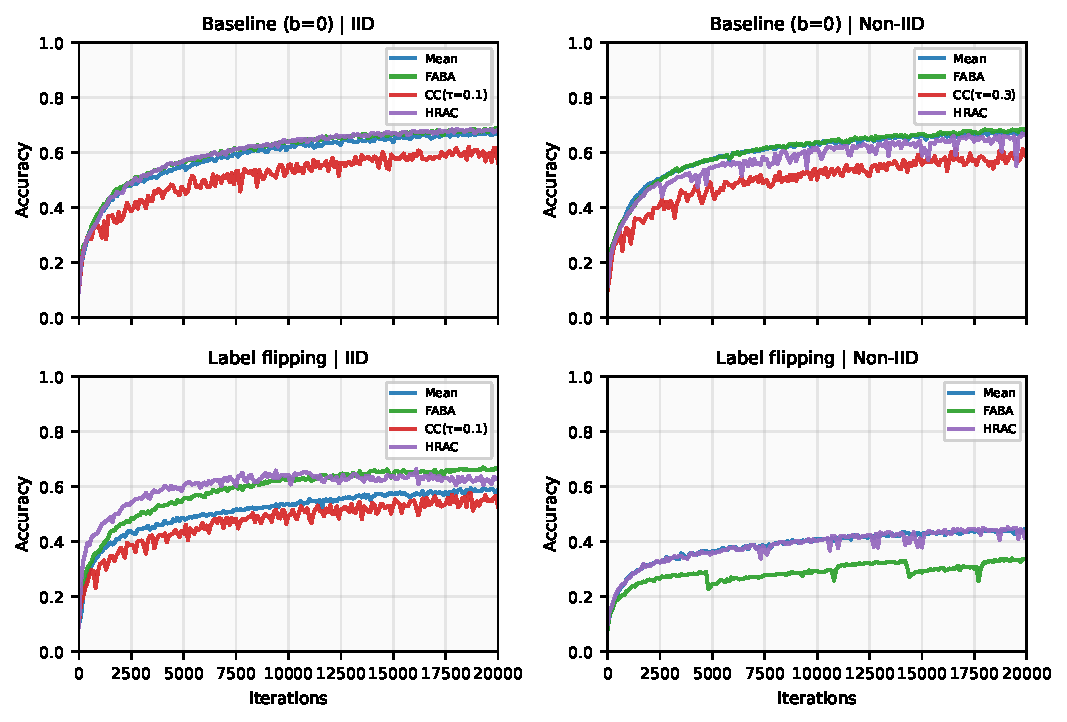
\includegraphics[width=\textwidth]{imgs/CMomentum_cifar10_b3_baseline_label_flipping}
    \caption{CIFAR-10 accuracy under benign training and label-flipping
    poisoning. The top row uses $b=0$; the label-flipping row uses $b=3$.}
    \label{fig:cifar10-baseline-label}
\end{figure}

Figure~\ref{fig:cifar10-msa-hismsa} shows attacks that manipulate update
structure or exploit temporal state. In the MSA panels, mean aggregation
degrades severely, especially under non-IID data, whereas HRAC maintains a much
higher trajectory. In the HisMSA panels, HRAC remains close to the best curves
and is particularly stable in the non-IID setting, which is consistent with the
design motivation for using client-specific history. These results show that
HRAC is most effective when the attack creates structured or persistent
deviation rather than only noisy benign variation.

\begin{figure}[p]
    \centering
    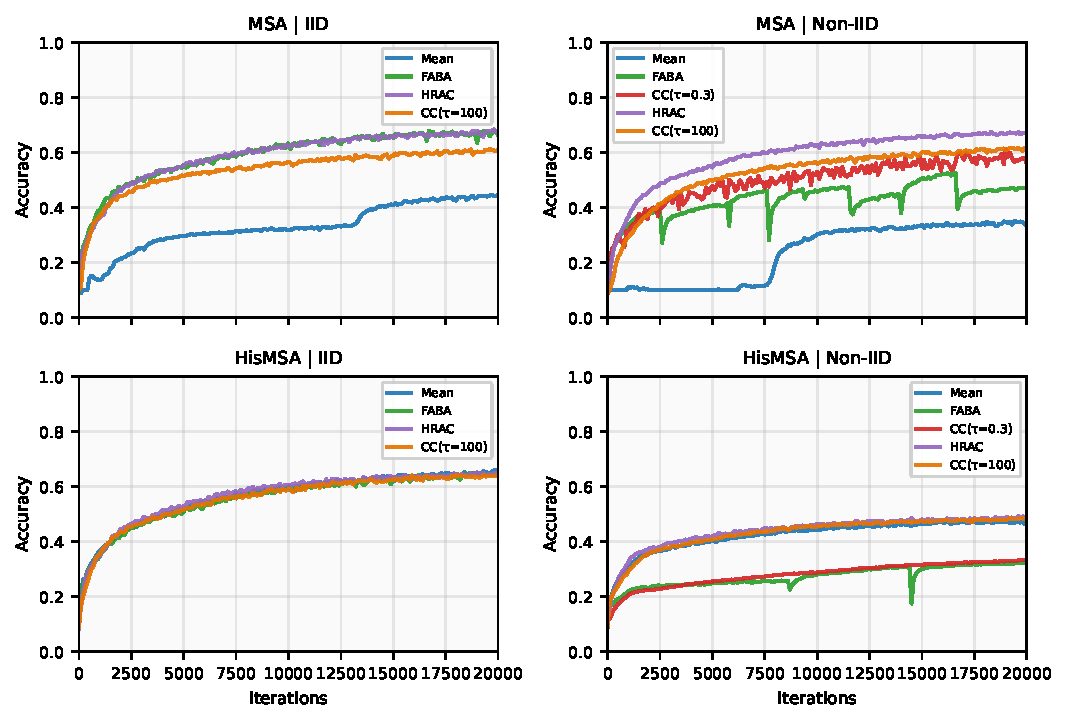
\includegraphics[width=\textwidth]{imgs/CMomentum_cifar10_b3_msa_hismsa}
    \caption{CIFAR-10 accuracy under model-shuffling (MSA) and history-aware
    model-shuffling (HisMSA) attacks with $b=3$.}
    \label{fig:cifar10-msa-hismsa}
\end{figure}

Figure~\ref{fig:cifar10-bit-alie-ipm} reports bit flipping, ALIE, and IPM. The
IID results are relatively close across several methods, but the non-IID panels
separate the defences more clearly. HRAC is consistently among the strongest
and most stable methods for non-IID ALIE and IPM. Bit flipping is more mixed in
the final-accuracy summaries: HRAC clearly suppresses the attackers in the
diagnostic plots, but FABA is higher by about five percentage points in the
non-IID $b=3$ final/best accuracy table. The centred-clipping
baseline also illustrates the limitation discussed in Chapter~\ref{ch2}: even
when used in the same baseline aggregation setting, a single centre is not a
reliable reference under the non-IID partition. Overall, the results support the
central design claim of HRAC: comparing clients against their own histories can
improve robustness to structured and history-aware attacks while preserving
benign training behaviour. At the same time, the mixed label-flipping and
bit-flipping panels show that HRAC should be treated as a robust aggregation
strategy rather than a universally dominant detector.

\begin{figure}[p]
    \centering
    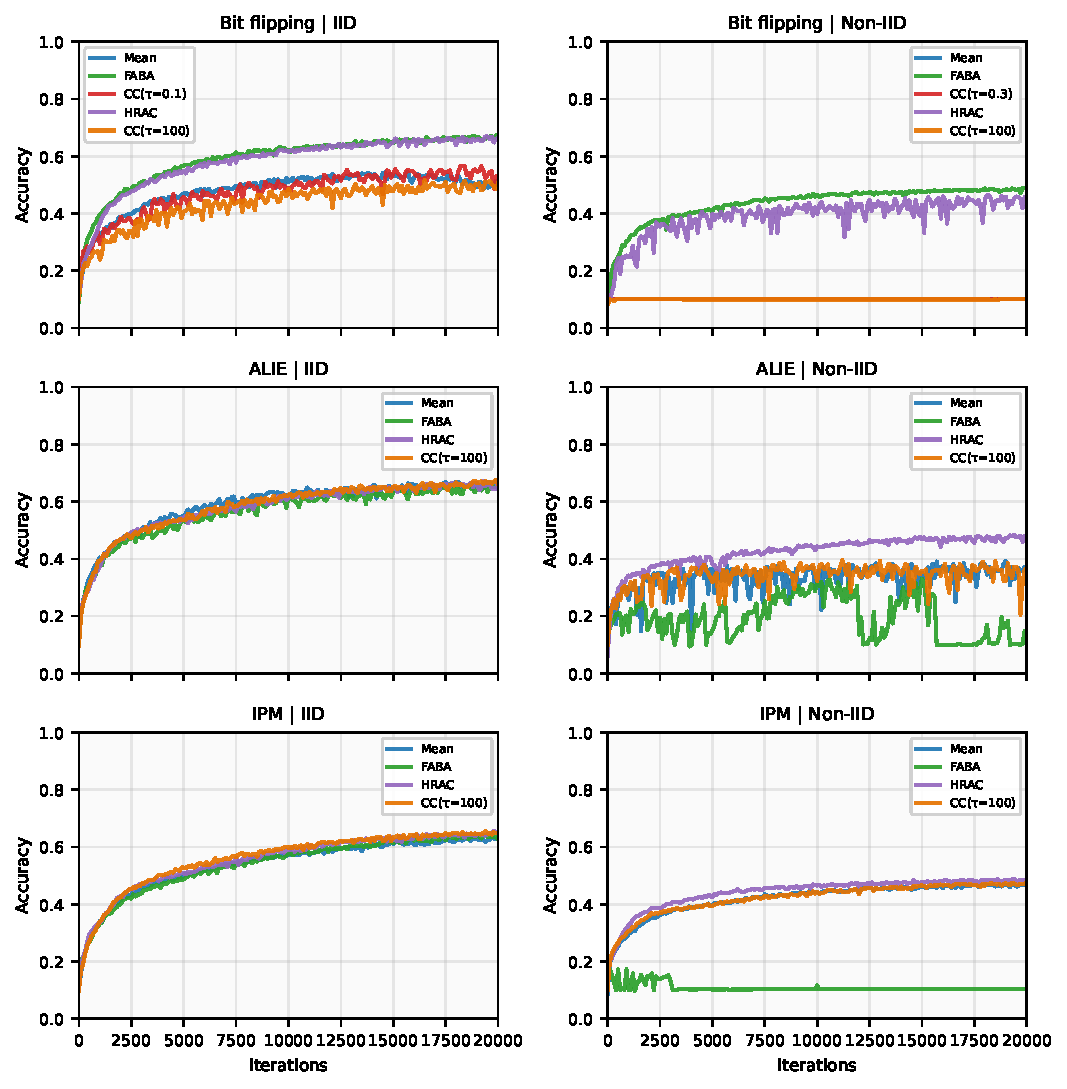
\includegraphics[width=\textwidth]{imgs/CMomentum_cifar10_b3_bit_alie_ipm}
    \caption{CIFAR-10 accuracy under bit-flipping, ALIE, and IPM attacks with
    $b=3$.}
    \label{fig:cifar10-bit-alie-ipm}
\end{figure}

Figures~\ref{fig:cifar10-b2-baseline-label}--\ref{fig:cifar10-b2-bit-alie-ipm}
repeat the same comparison with $b=2$. The lower attacker fraction reduces the
severity of several attacks, especially label flipping and ALIE, but the broad
pattern remains attack-dependent. Mean aggregation can recover in some
protocol-compliant data-poisoning settings. LFighter again remains competitive for IID label flipping but does not
resolve the non-IID label-flipping case. HRAC remains strongest in the
structured MSA setting and competitive in the remaining attacks.

\begin{figure}[p]
    \centering
    \includegraphics[width=\textwidth]{imgs/CMomentum_cifar10_b2_baseline_label_flipping}
    \caption{CIFAR-10 accuracy under benign training and label-flipping
    poisoning. The top row uses $b=0$; the label-flipping row uses $b=2$.}
    \label{fig:cifar10-b2-baseline-label}
\end{figure}

\begin{figure}[p]
    \centering
    \includegraphics[width=\textwidth]{imgs/CMomentum_cifar10_b2_msa_hismsa}
    \caption{CIFAR-10 accuracy under MSA and HisMSA attacks with $b=2$.}
    \label{fig:cifar10-b2-msa-hismsa}
\end{figure}

\begin{figure}[p]
    \centering
    \includegraphics[width=\textwidth]{imgs/CMomentum_cifar10_b2_bit_alie_ipm}
    \caption{CIFAR-10 accuracy under bit-flipping, ALIE, and IPM attacks with
    $b=2$.}
    \label{fig:cifar10-b2-bit-alie-ipm}
\end{figure}

\section{Additional Analyses}
\label{sec:additional-analyses}

Beyond the main comparison curves, the implementation was also used to isolate
which parts of HRAC are responsible for the observed behaviour. The component
study below is reported for non-IID CIFAR-10, where benign heterogeneity makes
hard filtering risky and where the main robustness claims are most relevant.
The remaining analysis focuses on what can be concluded from the available
logs, while broader sensitivity studies are treated as limitations and future
work.

\subsection{Final and Best Accuracy Summary}
\label{subsec:final-best-accuracy}

Tables~\ref{tab:final-best-accuracy} and \ref{tab:final-best-accuracy-b2}
complement the accuracy curves by reporting final-round and best observed test
accuracy. Each entry is written as ``final / best''. The best robust baseline
column is selected among FABA and CC, excluding both mean aggregation and HRAC,
so that mean aggregation remains visible as a separate reference. LFighter is
shown in the label-flipping curves but is not included in these summary tables
because cached LFighter runs are available only for label flipping, not for the
full attack suite.

\begin{table}[t]
    \centering
    \scriptsize
    \setlength{\tabcolsep}{3pt}
    \caption{Final and best CIFAR-10 test accuracy extracted from cached logs
    for the main $b=3$ attack setting. Entries are reported as final / best.}
    \label{tab:final-best-accuracy}
    \begin{tabular}{p{0.19\textwidth}p{0.13\textwidth}p{0.16\textwidth}p{0.24\textwidth}p{0.16\textwidth}}
        \hline
        \textbf{Setting} & \textbf{Partition} & \textbf{Mean} & \textbf{Best robust baseline} & \textbf{HRAC} \\
        \hline
        Baseline & IID & 0.6707 / 0.6780 & FABA: 0.6808 / 0.6887 & 0.6698 / 0.6721 \\
        Baseline & Non-IID & 0.6718 / 0.6770 & FABA: 0.6820 / 0.6857 & 0.6540 / 0.6839 \\
        Label flipping & IID & 0.5889 / 0.5951 & FABA: 0.6697 / 0.6697 & 0.6113 / 0.6152 \\
        Label flipping & Non-IID & 0.4391 / 0.4449 & CC: 0.3713 / 0.3794 & 0.4405 / 0.4429 \\
        MSA & IID & 0.4433 / 0.4464 & FABA: 0.6630 / 0.6789 & 0.6618 / 0.6618 \\
        MSA & Non-IID & 0.3369 / 0.3507 & CC: 0.5479 / 0.5626 & 0.6466 / 0.6466 \\
        HisMSA & IID & 0.6577 / 0.6593 & FABA: 0.6478 / 0.6500 & 0.6493 / 0.6732 \\
        HisMSA & Non-IID & 0.4734 / 0.4743 & CC: 0.4863 / 0.4868 & 0.4874 / 0.4912 \\
        Bit flipping & IID & 0.5006 / 0.5445 & FABA: 0.6687 / 0.6729 & 0.6685 / 0.6719 \\
        Bit flipping & Non-IID & 0.1000 / 0.1000 & FABA: 0.4875 / 0.4885 & 0.4371 / 0.4604 \\
        ALIE & IID & 0.6497 / 0.6758 & CC: 0.6607 / 0.6753 & 0.6662 / 0.6718 \\
        ALIE & Non-IID & 0.3585 / 0.3921 & CC: 0.3695 / 0.3953 & 0.4805 / 0.4846 \\
        IPM & IID & 0.6315 / 0.6348 & CC: 0.6512 / 0.6546 & 0.6459 / 0.6476 \\
        IPM & Non-IID & 0.4646 / 0.4733 & CC: 0.4736 / 0.4740 & 0.4839 / 0.4931 \\
        \hline
    \end{tabular}
\end{table}

\begin{table}[t]
    \centering
    \scriptsize
    \setlength{\tabcolsep}{3pt}
    \caption{Final and best CIFAR-10 test accuracy extracted from cached logs
    for the supplementary $b=2$ attack setting. Entries are reported as final /
    best.}
    \label{tab:final-best-accuracy-b2}
    \begin{tabular}{p{0.19\textwidth}p{0.13\textwidth}p{0.16\textwidth}p{0.24\textwidth}p{0.16\textwidth}}
        \hline
        \textbf{Setting} & \textbf{Partition} & \textbf{Mean} & \textbf{Best robust baseline} & \textbf{HRAC} \\
        \hline
        Label flipping & IID & 0.6330 / 0.6330 & FABA: 0.6638 / 0.6728 & 0.6494 / 0.6506 \\
        Label flipping & Non-IID & 0.5118 / 0.5264 & CC: 0.4461 / 0.4736 & 0.5215 / 0.5343 \\
        MSA & IID & 0.1000 / 0.1201 & FABA: 0.6544 / 0.6788 & 0.6785 / 0.6785 \\
        MSA & Non-IID & 0.1000 / 0.1000 & CC: 0.5780 / 0.5890 & 0.6628 / 0.6652 \\
        HisMSA & IID & 0.6725 / 0.6738 & FABA: 0.6615 / 0.6646 & 0.6629 / 0.6729 \\
        HisMSA & Non-IID & 0.5498 / 0.5498 & FABA: 0.4359 / 0.4363 & 0.5447 / 0.5472 \\
        Bit flipping & IID & 0.5640 / 0.5869 & FABA: 0.6642 / 0.6710 & 0.6665 / 0.6713 \\
        Bit flipping & Non-IID & 0.1000 / 0.1000 & FABA: 0.5544 / 0.5544 & 0.5227 / 0.5272 \\
        ALIE & IID & 0.6711 / 0.6711 & FABA: 0.6812 / 0.6852 & 0.6721 / 0.6721 \\
        ALIE & Non-IID & 0.5584 / 0.5618 & CC: 0.5522 / 0.5522 & 0.5571 / 0.5616 \\
        IPM & IID & 0.6601 / 0.6601 & CC: 0.6559 / 0.6667 & 0.6627 / 0.6753 \\
        IPM & Non-IID & 0.5443 / 0.5443 & CC: 0.5361 / 0.5388 & 0.5504 / 0.5565 \\
        \hline
    \end{tabular}
\end{table}

\subsection{Component Ablation Study}
\label{subsec:component-ablation}

The ablation study removes individual HRAC components while keeping the same
training setting. The tested variants remove the global median cap, remove
per-client residual clipping, remove $\nu$-based weighting, or keep only the
global cap before averaging. The goal is to check whether the observed behaviour
comes from one clipping rule or from the combination of scale control,
client-specific history, and temporal weighting.

The ALIE ablation in Figure~\ref{fig:alie-noniid-ablation} shows that the
global cap and residual clipping are not the decisive components in this run.
Both corresponding variants stay close to full HRAC
(Table~\ref{tab:alie-ablation}). In contrast, removing $\nu$ weighting causes a
large drop, and the global-cap-only variant performs similarly poorly. This
suggests that the residual-change statistic is the main useful signal against
ALIE in this experiment.

\begin{figure}[t]
    \centering
    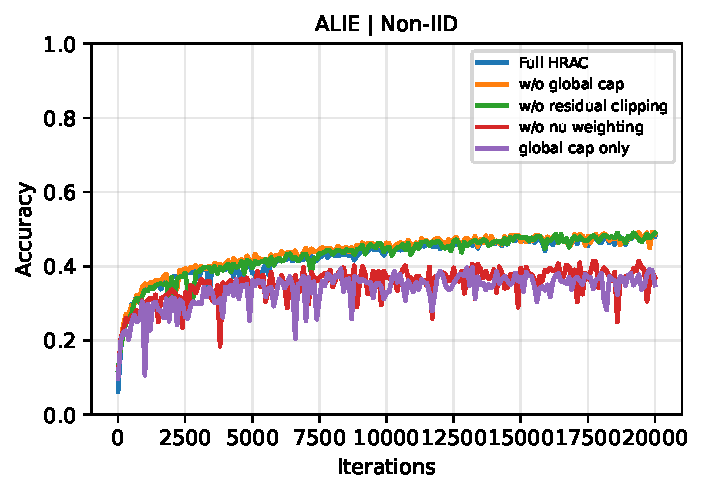
\includegraphics[width=0.82\textwidth]{imgs/CMomentum_cifar10_b3_ALIE_noniid_hrac_ablation}
    \caption{HRAC component ablation under ALIE on non-IID CIFAR-10 with
    $b=3$.}
    \label{fig:alie-noniid-ablation}
\end{figure}

\begin{table}[t]
    \centering
    \small
    \setlength{\tabcolsep}{4pt}
    \caption{Final and best test accuracy for the ALIE non-IID ablation study.}
    \label{tab:alie-ablation}
    \begin{tabular}{p{0.38\textwidth}p{0.18\textwidth}p{0.18\textwidth}p{0.18\textwidth}}
        \hline
        \textbf{Variant} & \textbf{Final} & \textbf{Best} & \textbf{Main effect} \\
        \hline
        Full HRAC & 0.4799 & 0.4843 & Reference method \\
        No global cap & 0.4863 & 0.4919 & Similar in ALIE \\
        No residual clipping & 0.4903 & 0.4903 & Similar in ALIE \\
        No $\nu$ weighting & 0.3691 & 0.4139 & Large degradation \\
        Global cap only & 0.3498 & 0.3979 & Large degradation \\
        \hline
    \end{tabular}
\end{table}

The MSA ablation in Figure~\ref{fig:msa-noniid-ablation} gives a different
pattern. Removing the global cap reduces accuracy to near chance level, while
removing residual clipping leaves a clear gap from full HRAC
(Table~\ref{tab:msa-ablation}). This indicates that MSA is controlled mainly by
explicit scale limitation, with residual clipping adding a second
history-aware constraint. The MSA ablation values come from a separate
controlled ablation cache rather than the main comparison cache used in
Table~\ref{tab:final-best-accuracy}, so the full-HRAC reference value is not
identical to the MSA entry in the main summary table.

\begin{figure}[t]
    \centering
    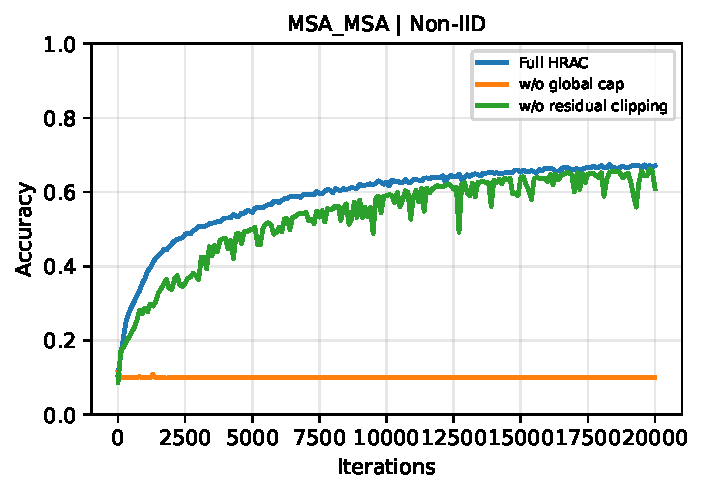
\includegraphics[width=0.82\textwidth]{imgs/CMomentum_cifar10_b3_MSA_MSA_noniid_hrac_ablation}
    \caption{HRAC component ablation under MSA on non-IID CIFAR-10 with
    $b=3$.}
    \label{fig:msa-noniid-ablation}
\end{figure}

\begin{table}[t]
    \centering
    \small
    \setlength{\tabcolsep}{4pt}
    \caption{Final and best test accuracy for the MSA non-IID ablation study.
    These controlled ablation runs use a separate cache from the main comparison
    in Table~\ref{tab:final-best-accuracy}; therefore the full-HRAC reference
    value differs from the main-table HRAC value.}
    \label{tab:msa-ablation}
    \begin{tabular}{p{0.42\textwidth}p{0.20\textwidth}p{0.20\textwidth}}
        \hline
        \textbf{Variant} & \textbf{Final} & \textbf{Best} \\
        \hline
        Full HRAC & 0.6713 & 0.6743 \\
        No global cap & 0.1000 & 0.1163 \\
        No residual clipping & 0.6099 & 0.6615 \\
        \hline
    \end{tabular}
\end{table}

Overall, the ablations show that HRAC's components matter in different ways for
different attacks. Temporal weighting is most useful for ALIE, while the global
cap is essential for MSA and residual clipping gives additional protection. This
supports keeping the three mechanisms together rather than treating HRAC as a
single clipping heuristic.

\subsection{Diagnostic Analysis}
\label{subsec:diagnostic-analysis}

The HRAC logs also allow the accuracy results to be connected to the internal
statistics used by HRAC. During training, the implementation records
per-round residual thresholds $\tau_i$, residual scale statistics $\mu_i$,
residual-change statistics $\nu_i$, normalised client weights, pre- and
post-clipping norms, and bottom-weight summaries for controlled simulation
runs.

The diagnostic plots are treated as supporting analysis rather than as the
primary evidence for HRAC. The left panel tracks the average residual-change
statistic $\nu_i$ for benign and Byzantine clients, the middle panel shows their
normalised aggregation weights, and the right panel counts how many Byzantine
clients appear among the three lowest-weighted clients. The main empirical
claims in this chapter therefore rest on the accuracy curves, final/best
accuracy summaries, and component ablations, while diagnostics are used to
interpret those results.

Across most attacks, these diagnostics show the intended behaviour. Once the
weighting stage becomes active, Byzantine clients tend to have larger
residual-change statistics, receive lower average weights, and appear
frequently in the bottom-weight set. This pattern is visible for bit flipping,
ALIE, IPM, HisMSA, and IID label flipping. It suggests that the weighting rule
is often suppressing the clients that generate abnormal residual dynamics.

The weaker cases are also informative. For MSA, strong accuracy does not always
come with clean attacker identification in the weight diagnostics. This is
consistent with the ablation result, where the global cap is the decisive
component and limits the effect of shuffled or amplified updates even when the
weights are not a reliable detector. For label flipping, the IID case still
shows clear attacker down-weighting, but the non-IID case is harder. Benign
label-skew already creates client-specific residual variation, so poisoned and
benign $\nu_i$ trajectories overlap more strongly and the bottom-weight summary
captures the attackers less consistently. This is why protocol-compliant label
poisoning becomes more difficult when it is combined with heterogeneous data.

\begin{figure}[p]
    \centering
    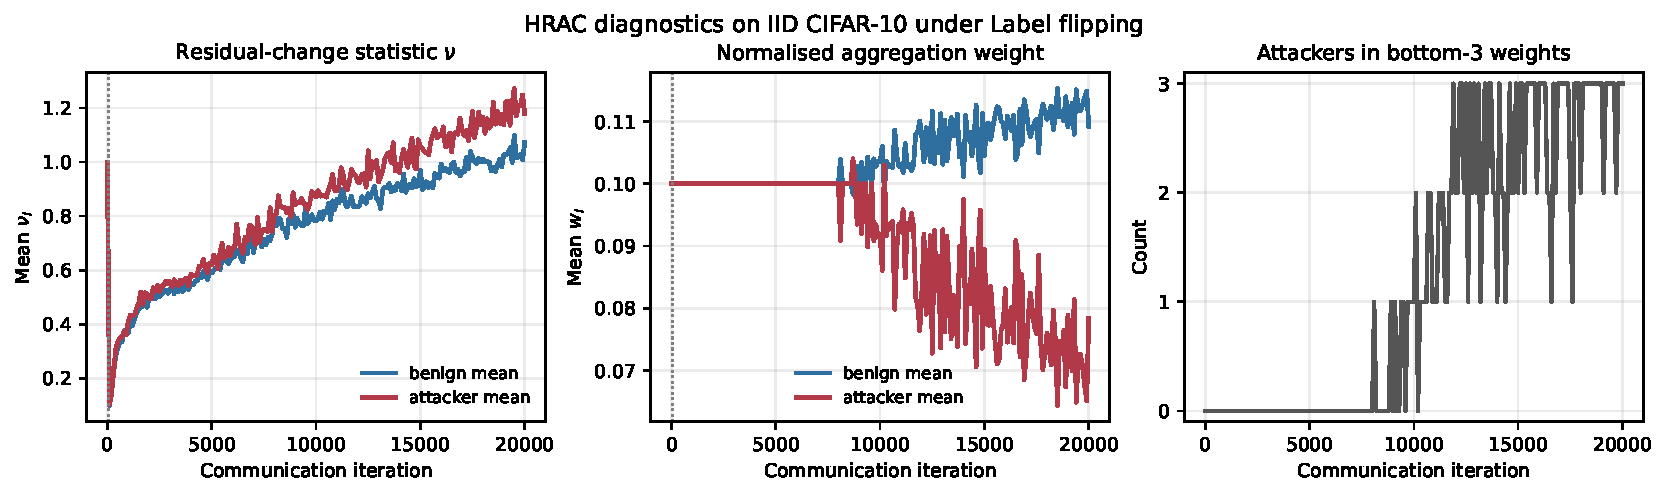
\includegraphics[width=\textwidth]{imgs/hrac_diagnostics_all_attacks/HRAC_diagnostics_label_flipping_iid}
    \vspace{0.5em}
    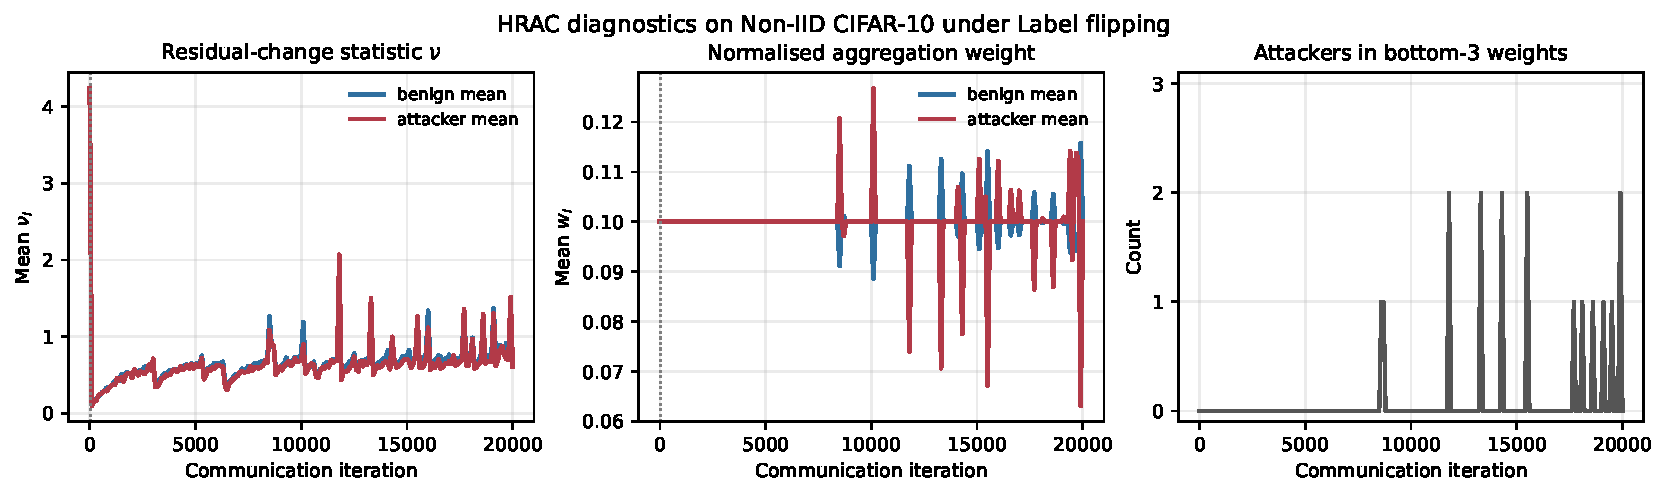
\includegraphics[width=\textwidth]{imgs/hrac_diagnostics_all_attacks/HRAC_diagnostics_label_flipping_noniid}
    \caption{HRAC diagnostics under label-flipping attacks for IID and non-IID
    CIFAR-10.}
    \label{fig:diag-label-flipping}
\end{figure}

\begin{figure}[p]
    \centering
    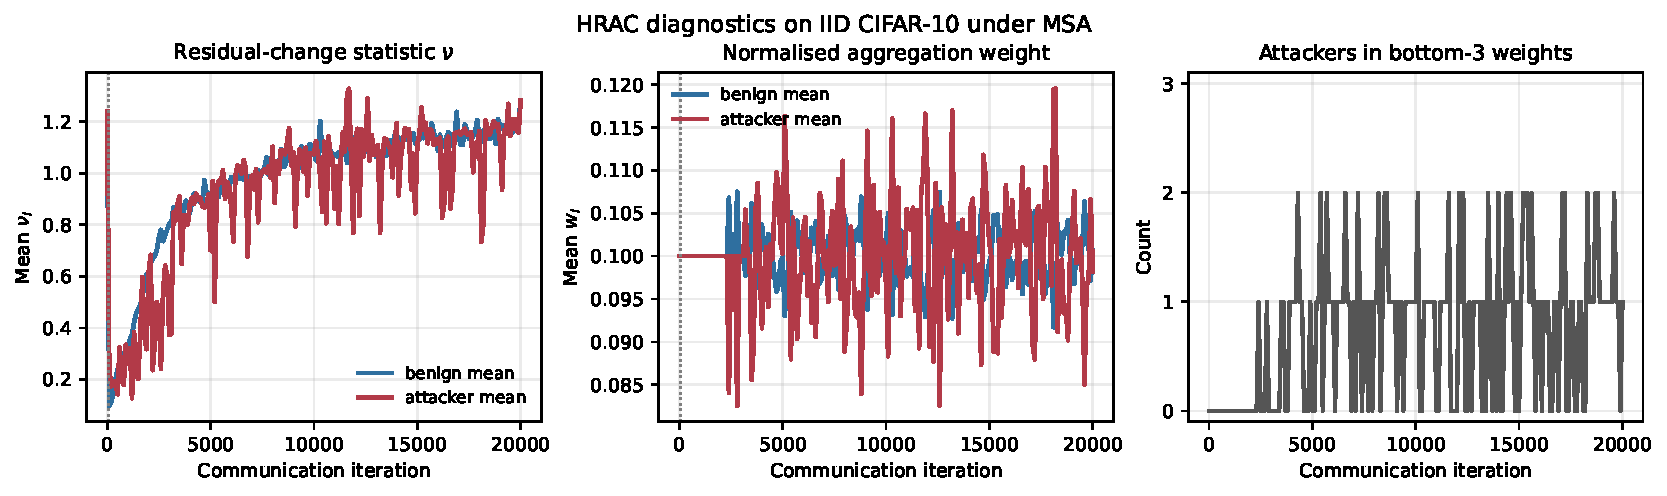
\includegraphics[width=\textwidth]{imgs/hrac_diagnostics_all_attacks/HRAC_diagnostics_MSA_iid}
    \vspace{0.5em}
    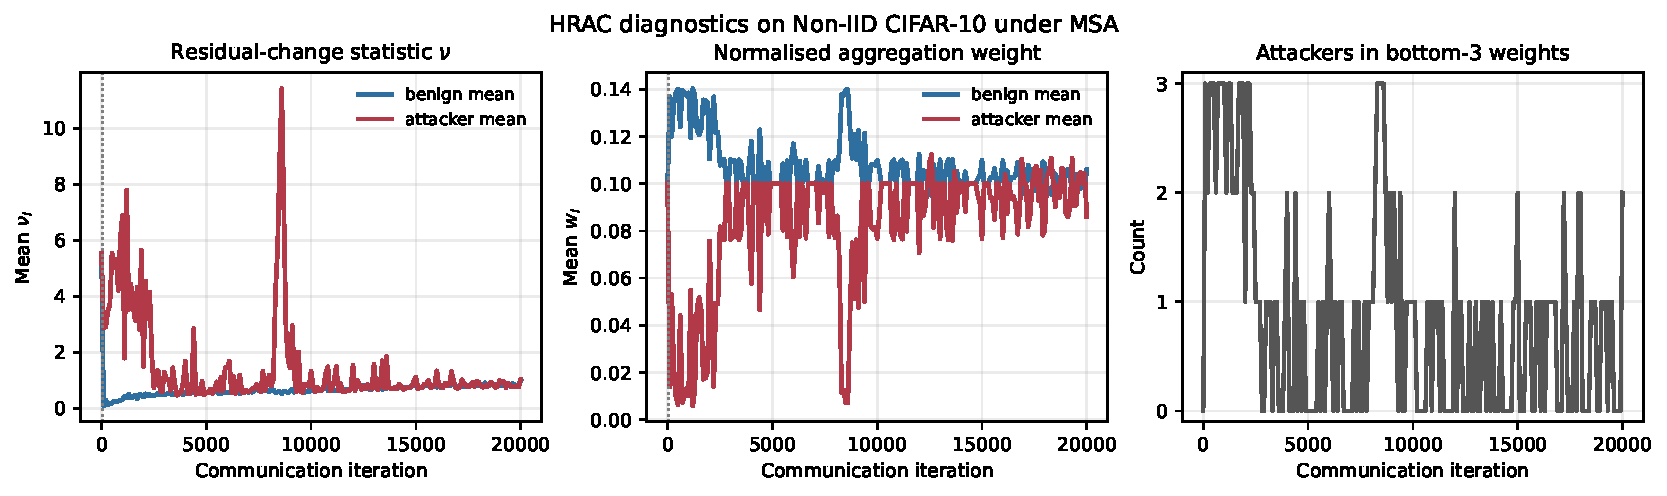
\includegraphics[width=\textwidth]{imgs/hrac_diagnostics_all_attacks/HRAC_diagnostics_MSA_noniid}
    \caption{HRAC diagnostics under MSA attacks for IID and non-IID CIFAR-10.}
    \label{fig:diag-msa}
\end{figure}

\begin{figure}[p]
    \centering
    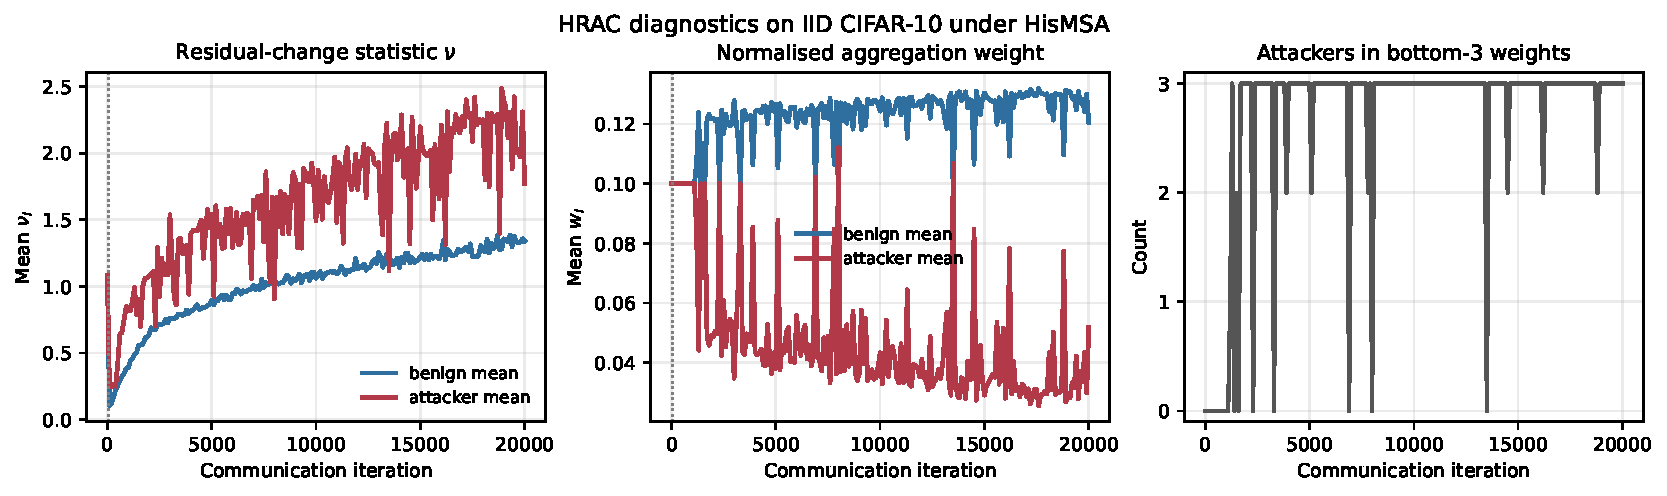
\includegraphics[width=\textwidth]{imgs/hrac_diagnostics_all_attacks/HRAC_diagnostics_HisMSA_iid}
    \vspace{0.5em}
    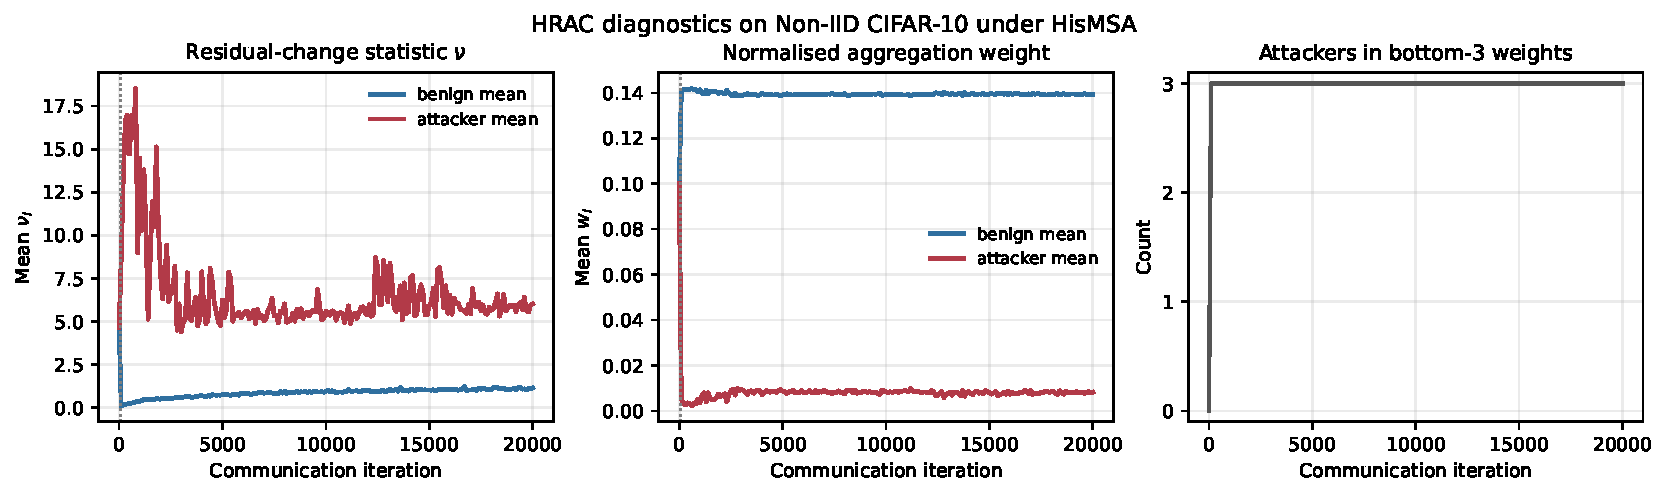
\includegraphics[width=\textwidth]{imgs/hrac_diagnostics_all_attacks/HRAC_diagnostics_HisMSA_noniid}
    \caption{HRAC diagnostics under HisMSA attacks for IID and non-IID
    CIFAR-10.}
    \label{fig:diag-hismsa}
\end{figure}

\begin{figure}[p]
    \centering
    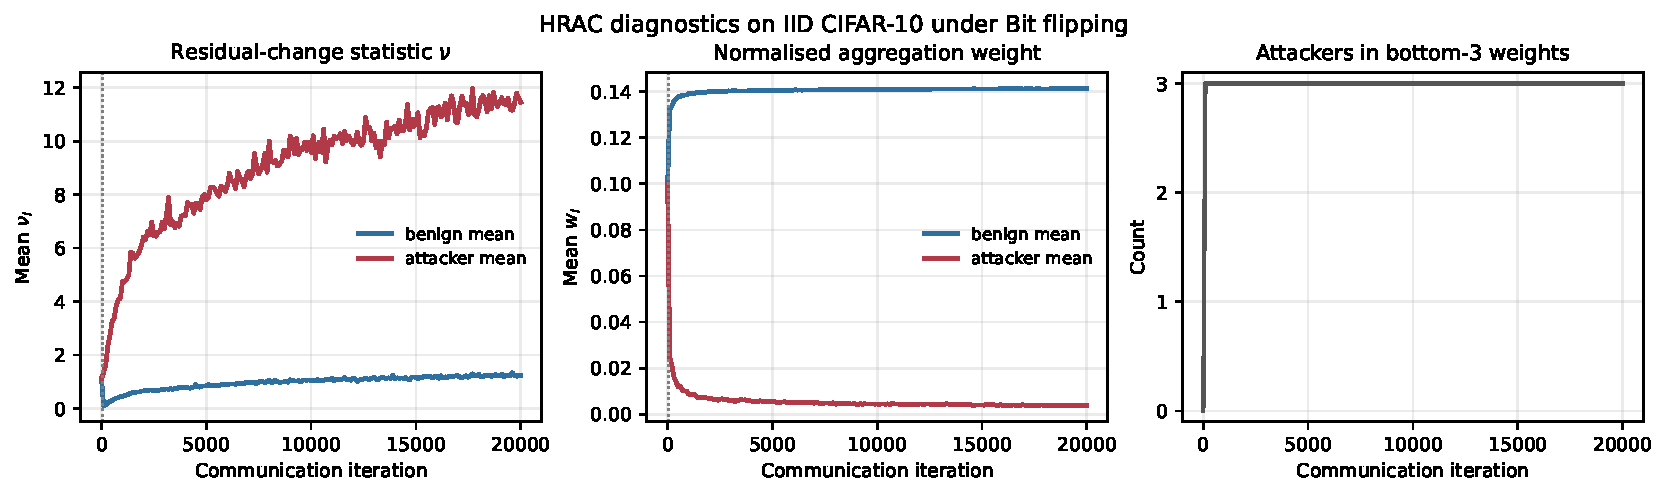
\includegraphics[width=\textwidth]{imgs/hrac_diagnostics_all_attacks/HRAC_diagnostics_bit_flipping_iid}
    \vspace{0.5em}
    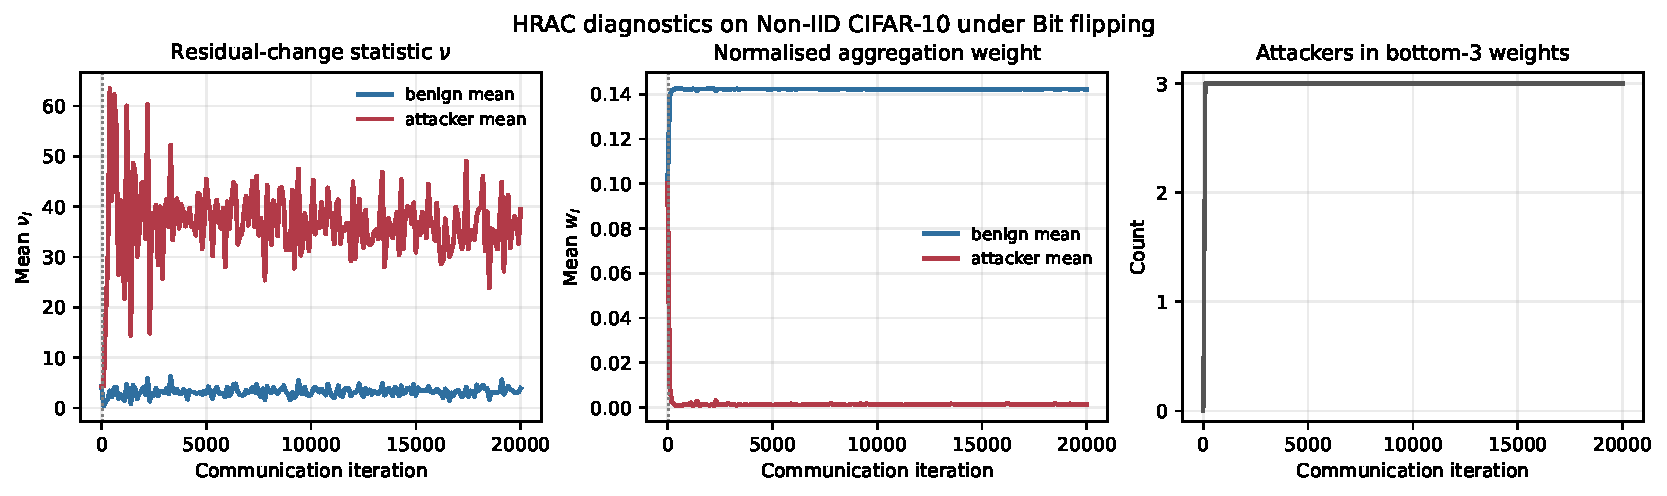
\includegraphics[width=\textwidth]{imgs/hrac_diagnostics_all_attacks/HRAC_diagnostics_bit_flipping_noniid}
    \caption{HRAC diagnostics under bit-flipping attacks for IID and non-IID
    CIFAR-10.}
    \label{fig:diag-bit-flipping}
\end{figure}

\begin{figure}[p]
    \centering
    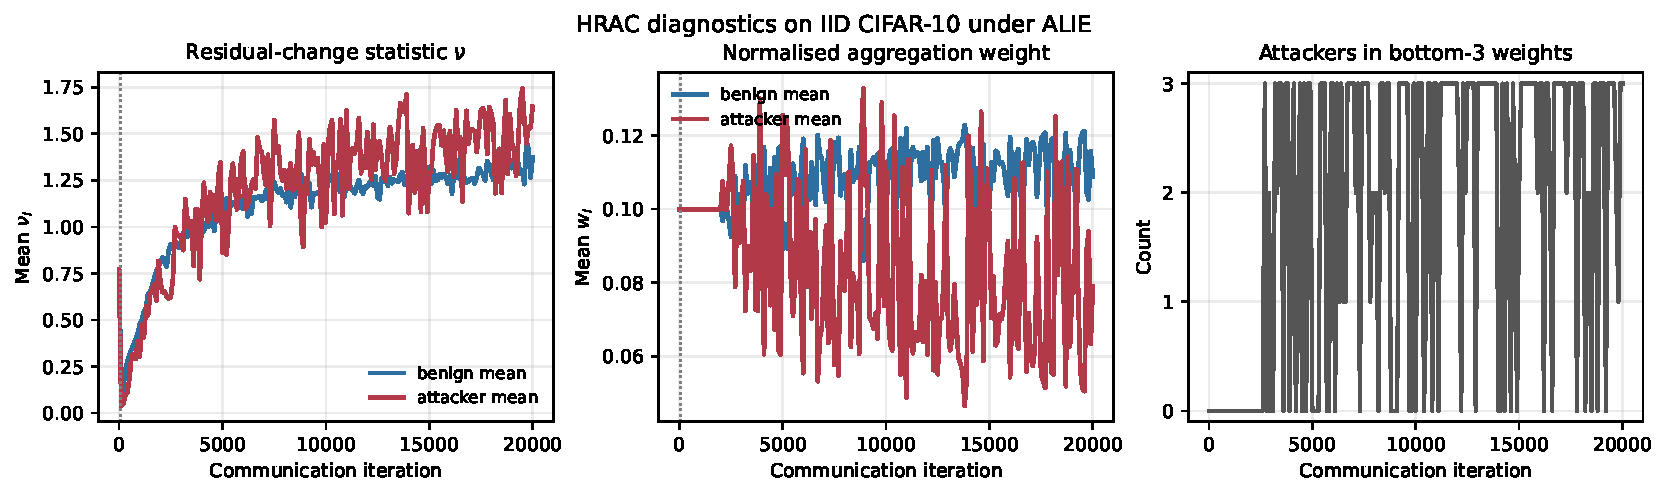
\includegraphics[width=\textwidth]{imgs/hrac_diagnostics_all_attacks/HRAC_diagnostics_ALIE_iid}
    \vspace{0.5em}
    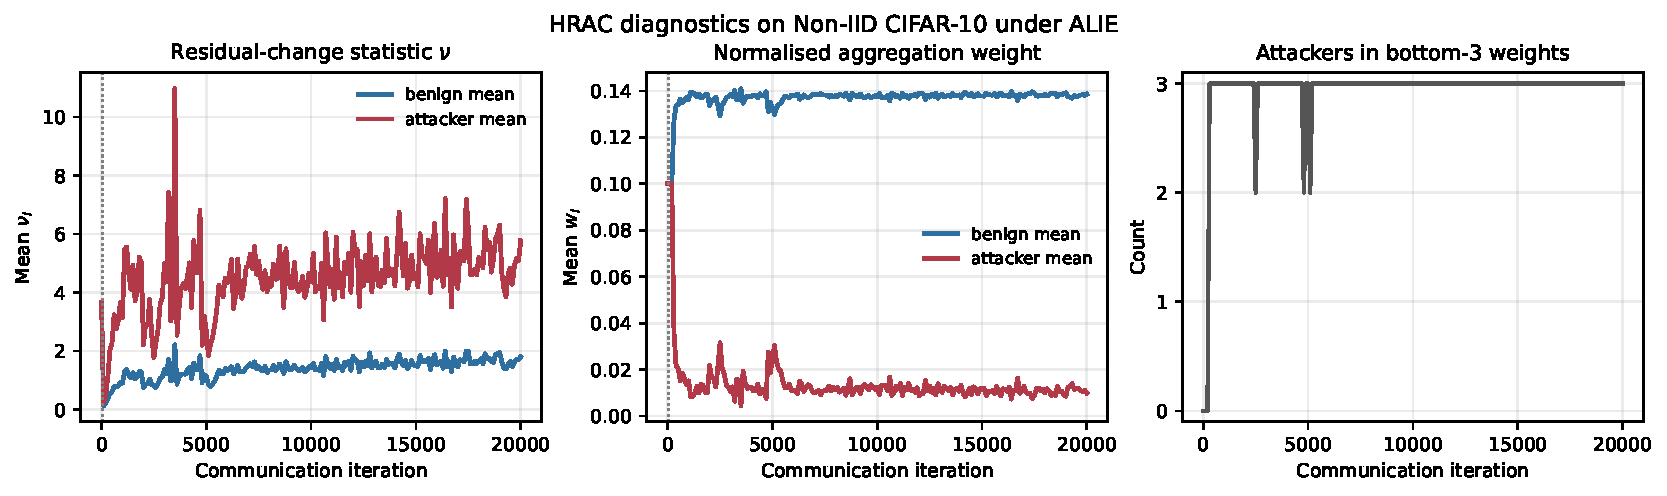
\includegraphics[width=\textwidth]{imgs/hrac_diagnostics_all_attacks/HRAC_diagnostics_ALIE_noniid}
    \caption{HRAC diagnostics under ALIE attacks for IID and non-IID CIFAR-10.}
    \label{fig:diag-alie}
\end{figure}

\begin{figure}[p]
    \centering
    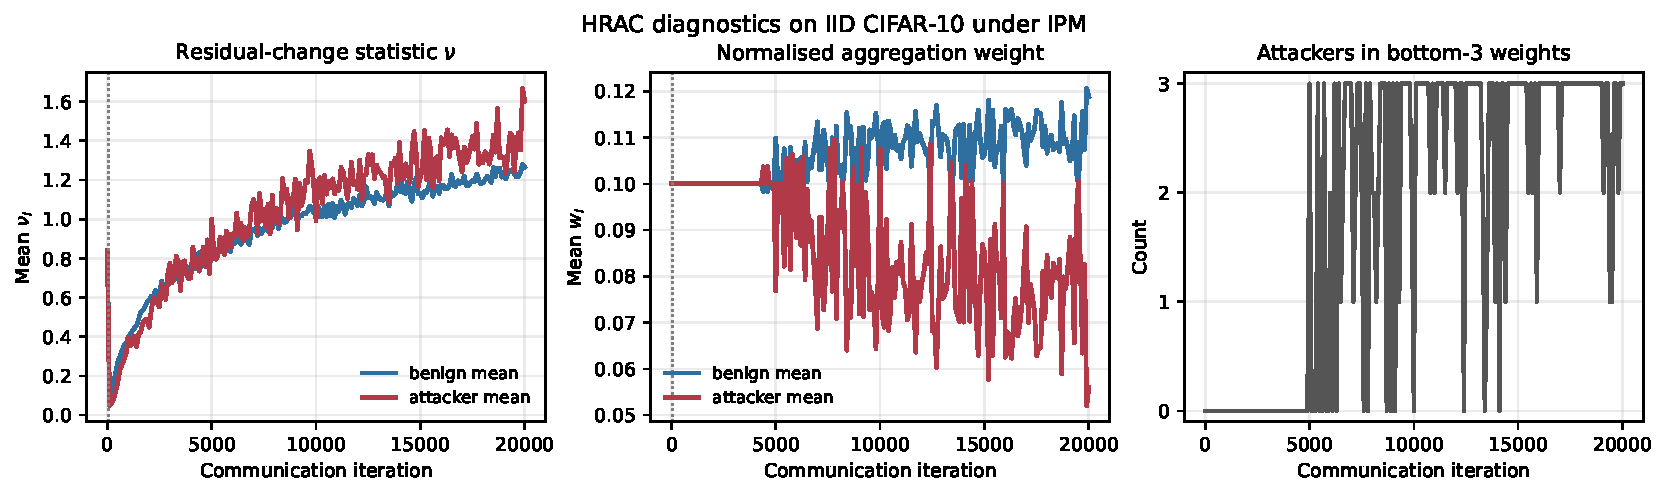
\includegraphics[width=\textwidth]{imgs/hrac_diagnostics_all_attacks/HRAC_diagnostics_IPM_iid}
    \vspace{0.5em}
    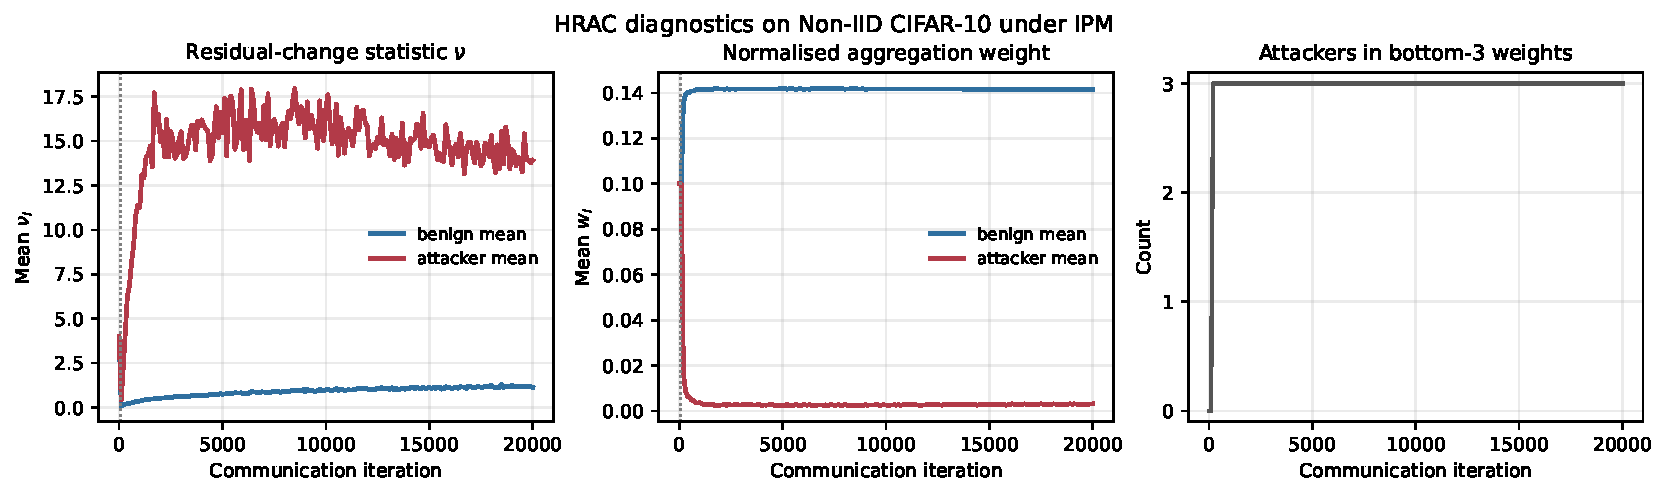
\includegraphics[width=\textwidth]{imgs/hrac_diagnostics_all_attacks/HRAC_diagnostics_IPM_noniid}
    \caption{HRAC diagnostics under IPM attacks for IID and non-IID CIFAR-10.}
    \label{fig:diag-ipm}
\end{figure}

\section{Discussion and Limitations}
\label{sec:discussion-limitations}

The experimental results match the trade-off stated in the abstract. Mean
aggregation can remain competitive for protocol-compliant poisoning under
heterogeneous data, but it is not reliable under stronger model-poisoning
attacks. Some robust baselines are
strong in particular cases, but their relative ranking changes with the attack
and partition. HRAC is most useful when malicious behaviour appears as
structured or persistent deviation, as in MSA, HisMSA, non-IID ALIE, and
non-IID IPM.

The mixed label-flipping and bit-flipping results are therefore part of the
claim rather than an exception to it. Under IID label flipping, HRAC performs
well because poisoned clients stand out more clearly from a relatively aligned
benign population. The diagnostic plot supports this because attacker weights
decline over training, and the bottom-weight set increasingly contains the
Byzantine clients. Under non-IID label flipping, the difficulty comes from the
interaction between the attack and the data partition rather than from label
flipping alone. Benign label-skew already produces client-specific residual
variation, so the $\nu$ trajectories of benign and poisoned clients overlap
much more, and the bottom-weight summary captures the attackers less
consistently. LFighter follows a similar pattern in the available
label-flipping runs, where it is strong under IID data but weaker under the
non-IID partition. Bit flipping is different: in the diagnostic plots, the
attacker $\nu$ values separate strongly from the benign clients, the attacker
weights are pushed close to zero, and the bottom-weight summary consistently
contains the Byzantine clients. HRAC should therefore be read as a balanced
robust aggregation strategy, not as a specialised label-poisoning defence.

The main limitations are the fixed HRAC hyperparameter setting and the
restricted experiment grid. The current cached results use CIFAR-10, \(N=10\)
clients, seed 100, \(b=2\) and \(b=3\) attack settings, and one label class per
client for the non-IID partition. The attack parameters are also fixed in the
reported runs, for example IPM uses \(\epsilon=0.1\) and MSA/HisMSA use shuffle
probability 1.0 with scaling range \((0.1,10.0)\). A stronger empirical study
would rerun the same comparison across multiple seeds, datasets, client counts,
attacker fractions, label-skew severities, and attack strengths.
